\documentclass[12pt,a4paper]{article}
\usepackage[utf8]{inputenc}
\usepackage[german]{babel}
\usepackage[T1]{fontenc}
\usepackage{amsmath}
\usepackage{amsfonts}
\usepackage{amssymb}
\usepackage{graphicx}
\usepackage{hyperref}\usepackage[left=2cm,right=2cm,top=2cm,bottom=2cm]{geometry}
\usepackage[dvipsnames]{xcolor}
\author{Gerhard Hofmann}
\title{Simulation eines Nahwärmesystems mit solarthermischer Energiequelle und Erdsonden-Wärmespeicher}
\begin{document}
\maketitle
\tableofcontents
\section{Kurzfassung}
Nahwärmesysteme mit solarthermischer Energiequelle und Erdsonden-Wärmespeicher sind ein vielversprechendes Konzept für die Wärmewende, d.h. für die Wärmeversorgung von Büro- und Wohnhäusern ohne fossile Brennstoffe und mit minimalem Stromeinsatz.\\
Ein solches System besteht aus mehreren Komponenten, die gut aufeinander abgestimmt sein müssen. Als Komponenten betrachten wir:\begin{itemize}
\item Solarthermiefeld
\item Erdsonden-Wärmespeicher
\item Pufferspeicher
\item Wärmeverbraucher
\item Hausübergabestation
\item Nahwärmeleitungen
\item Wärmepumpen
\end{itemize}
Manche dieser Komponenten sind in einem bestimmten Szenario bereits vorgegeben, andere müssen noch dimensioniert werden. 
Es wird angestrebt, eine möglichst hohe solare Deckungsrate bei der Wärmeversorgung zu erreichen. Dazu kann man mit der hier vorgestellten Software \texttt{DistrictHeating} die verschiedenen noch freien Parameter (z.B. Abstand der Erdsonden zueinander, Vorlauftemperatur im Netz u.v.m.) variieren und nach einer Simulation über den Jahresverlauf z.B. den Stromverbrauch der Wärmepumpen feststellen.\\
Angeregt wurde die Entwicklung der Simulation \texttt{DistrictHeating} durch die Dissertation \emph{\glqq Object-oriented modelling of solar district heating grids with underground thermal energy storage\grqq} \footnote{\url{https://tubiblio.ulb.tu-darmstadt.de/133074/}} von Julian Formhals, in der die Simulation eines ebensolchen Nahwärmesystems basierend auf Modelica beschrieben wird. Diese Simulation von Julian Formhals ist weitaus realistischer als \texttt{DistrictHeating}, benötigt jedoch auch wesentlich mehr Rechenzeit. Somit ist es kaum möglich mehrere Parameter über Testreihen zu verändern um eine optimale Konfiguration zu finden.
\section{Einleitung}
Das \texttt{DistrictHeating} zugrunde liegende physikalische Konzept besteht aus einem Nahwärme-Leitungsnetz mit zwei oder drei Leitungen, die in der Straße verlegt werden und an die die verschiedenen Komponenten angeschlossen sind. Die einzelnen Komponenten können dem Netz Wärme entziehen oder Wärme zuführen.
\section{Die Simulation}
\texttt{DistrictHeating} ist in \texttt{C\#} geschrieben und läuft unter .NET. Die Applikation enthält eine Benutzeroberfläche, mit deren Hilfe die Komponenten zusammengestellt und definiert werden können. Die Möglichkeiten sind weit entfernt von dem, was in Modelica möglich ist. Es ist vielmehr genau zugeschnitten auf eine Anlage mit einem Solarthermiefeld, einem Erdsonden-Wärmespeicher, einem Pufferspeicher, verschiedenen Wärmeverbrauchern, Nahwärmeleitungen und Wärmepumpen.
\subsection{Komponenten} Die einzelnen Komponenten sind als Klassen implementiert. Im wesentlichen ist es die Aufgabe der Komponenten zu einem gegebenen Zeitpunkt zu berechnen, mit welcher Leistung dem System gerade Energie zugeführt oder entnommen wird und wie viel zusätzlicher Strom (z.B. für eine Wärmepumpe) verwendet wird. Dazu muss die Komponente folgende Werte bestimmen:
\begin{description}
\item[Volumenstrom (\texttt{out double volumetricFlowRate}) in $\frac{m^3}{s}$]
\item[Temperaturdifferenz (\texttt{out double deltaT}) in $K$]
\item[Eingangsleitung (\texttt{out Pipe fromPipe})]
\item[Ausgangsleitung (\texttt{out Pipe toPipe})]
\item[Elektrische Leistung (\texttt{out double electricPower}) in $W$]
\end{description}
\texttt{Pipe} ist einer der folgenden Werte: \texttt{enum Pipe \{ returnPipe, warmPipe, hotPipe \}}.
Es sind Anlagen simulierbar mit zwei Leitungen (warmer Vorlauf und kalter Rücklauf für Verbraucher, für Erzeuger ist die Richtung umgekehrt) oder drei Leitungen (im Winter zwei verschiedene Temperaturen für Vorlauf, der wärmere für Warmwasser und Heizkörperheizung mit garantierten 50°C, im Sommer 50°C für Warmwasser und 5°C zum Kühlen, und jeweils ein Rücklauf). Im Dreileitungssystem entscheidet die Komponente, aus welcher Leitung sie das Wasser zieht und in welche Leitung sie das thermisch veränderte Wasser wieder abgibt.
Die Leistung wird definiert durch einen Volumenstrom $\frac{m^3}{s}$ des Wärmeträgers (Wassers) in den Leitungen und einer Temperaturdifferenz $\Delta T$ zwischen dem entnommenen und dem wieder zugeführten Wasser.
\subsection{Die Anlage (\texttt{class Plant})}
Die Anlage (\texttt{class Plant}) ist das zentrale und singuläre Objekt der Simulation. Sie ist selbst keine Komponente. Sie kennt den Zustand der Leitungen, d.h. die Temperatur des Wassers in den Leitungen. Darüber hinaus kennt sie den Zeitpunkt, an dem sich die Simulation gerade befindet und hält eine Liste aller Komponenten.\\
Die Simulation fragt alle Komponenten der Reihe nach ab, mit welcher Leistung sie gerade arbeiten und verändert entsprechend die Temperatur im Leitungsnetz. Die Geometrie des Leitungsnetzes, also an welcher Stelle die einzelnen Komponenten angeschlossen sind, oder die Auslegung als Ring oder Netz, wird nicht berücksichtigt. Lediglich die Länge, das Wasservolumen und die Dämmwerte sind gegeben und werden entsprechend berücksichtigt.
\subsection{Die Heizung (\texttt{class HeatingConsumer})}
Die Heizung (\texttt{class HeatingConsumer}) ist der typische Wärmeverbraucher. In ihrer Definition sind folgende Eigenschaften gesetzt:
\begin{description}
\item[Vorlauftemperatur (\texttt{double[] SupplyTemp}):] acht Werte, die die Vorlauftemperatur zwischen -20°C und +20°C in 5° Schritten definieren. Zwischenwerte werden interpoliert.
\item[Gesamtverbrauch pro Jahr (\texttt{double PowerConsumptionPerYear}) in $J$.]
\item[Die Temperaturen (\texttt{double DayTemperature, double NightTemperature}):] die gewünschte Raumtemperatur.
\item[Nachtabsenkung (\texttt{int DayStartHour, int DayEndHour}):]
 Start- und Endzeit für die Tagestemperatur. Dazwischen ist Nachtabsenkung.
\item[Gütegrad der Wärmepumpe (\texttt{double HeatPumpEfficiency}):]
Die Effizienz der Wärmepumpe, die zum Einsatz kommt, wenn die Temperatur aus dem Nahwärmenetz kleiner ist als die gewünschte Vorlauftemperatur.
\end{description}
Die Heizung greift auf die Wetterdaten zu. Die benötigte Leistung wird proportional zur Differenz aus Vorlauftemperatur und der Außentemperatur gesetzt. Der Faktor für die Proportionalität wird  so bestimmt, dass der Jahresverbrauch den vorgegebenen Wert erreicht. Zum Test habe ich aus den Wetterdaten des DWD \footnote{Deutscher Wetterdienst, Klimadaten zum direkten Download (Gießen/Wettenberg) \url{https://opendata.dwd.de/climate_environment/CDC/observations_germany/}} die monatlichen Verbräuche bestimmt und mit den zu erwartenden gemäß \emph{statista}\footnote{siehe Struktur des jährlichen Erdgasverbrauchs in deutschen Haushalten nach Monaten \url{https://de.statista.com/statistik/daten/studie/160067/umfrage/verbrauch-von-heizenergie-nach-monaten/}} verglichen. Siehe Tabelle \ref{Monatsverbrauch}
\begin{table}[h]\scriptsize \centering
\begin{tabular}[h]{c|c|c|c|c|c|c|c|c|c|c|c|c}
Jahr & Jan & Feb & Mär & Apr & Mai & Jun & Jul & Aug & Sep & Okt & Nov & Dez \\
\hline
Avg & 16.1 & 13 & 12.5 & 8.1 & 3.5 & 2.2 & 1.7 & 1.6 & 5.2 & 8.4 & 12.2 & 15.5 \\
\hline
2000 & 16\% & 13.1\% & 12.2\% & 8.2\% & 3.8\% & 2.8\% & 3.1\% & 0.8\% & 4.7\% & 8.2\% & 12.2\% & 14.8\% \\
2001 & 15.6\% & 12.7\% & 12\% & 9.6\% & 3.3\% & 4\% & 1\% & 0.9\% & 6.3\% & 6\% & 13.1\% & 15.6\% \\
2002 & 15.5\% & 12\% & 12.2\% & 9.3\% & 5.1\% & 1.5\% & 1.5\% & 0.7\% & 5.6\% & 9.5\% & 12\% & 15.1\% \\
2003 & 16.3\% & 15.6\% & 10.9\% & 8.5\% & 4.3\% & 0.9\% & 0.6\% & 0.7\% & 4.9\% & 10.7\% & 10.8\% & 15.6\% \\
2004 & 14.9\% & 12.8\% & 12.5\% & 7.9\% & 5.9\% & 3.1\% & 1.8\% & 1.2\% & 3.8\% & 7.7\% & 12.5\% & 15.9\% \\
2005 & 14.6\% & 15.7\% & 11.8\% & 7.6\% & 5.5\% & 2.6\% & 1.4\% & 2\% & 4\% & 7\% & 12.4\% & 15.3\% \\
2006 & 17.9\% & 14.4\% & 14.7\% & 9.6\% & 5.1\% & 2.8\% & 0.2\% & 3.6\% & 2.5\% & 6.1\% & 10\% & 13.2\% \\
2007 & 12.6\% & 13\% & 11.9\% & 6.3\% & 4.2\% & 2.1\% & 2.5\% & 2.3\% & 6.1\% & 9.7\% & 13.4\% & 16\% \\
2008 & 13.1\% & 12.8\% & 12.8\% & 9.8\% & 3.5\% & 2.3\% & 1.5\% & 1.4\% & 6.2\% & 9.1\% & 12.1\% & 15.4\% \\
2009 & 18.1\% & 13.7\% & 12.2\% & 6.5\% & 4.5\% & 4.4\% & 1.1\% & 1.2\% & 3.9\% & 9\% & 9.9\% & 15.4\% \\
2010 & 16\% & 12.9\% & 11.1\% & 7.3\% & 6.7\% & 2.3\% & 0.7\% & 2.1\% & 5.3\% & 8.6\% & 10.6\% & 16.5\% \\
2011 & 15.2\% & 14.1\% & 11.8\% & 6.3\% & 4.5\% & 3\% & 2.6\% & 1.7\% & 4.6\% & 9.3\% & 13.3\% & 13.6\% \\
2012 & 14.8\% & 15.4\% & 10.1\% & 8.8\% & 4.1\% & 3.3\% & 2\% & 1.1\% & 5.6\% & 9.3\% & 11.9\% & 13.6\% \\
2013 & 15.3\% & 14.4\% & 14.7\% & 8.3\% & 6.3\% & 3.4\% & 0.5\% & 1.2\% & 4.6\% & 6.8\% & 12\% & 12.4\% \\
2014 & 14.9\% & 13\% & 11.6\% & 7.3\% & 6.2\% & 3.8\% & 0.8\% & 3.4\% & 3.6\% & 7.2\% & 12.5\% & 15.6\% \\
2015 & 15\% & 14.5\% & 12.8\% & 8.8\% & 6\% & 2.7\% & 1.1\% & 1.1\% & 5.4\% & 9.7\% & 11\% & 11.9\% \\
2016 & 14.5\% & 12.9\% & 13.3\% & 9.8\% & 4.4\% & 2.5\% & 1.1\% & 1.2\% & 2.7\% & 9\% & 13.1\% & 15.5\% \\
2017 & 17.9\% & 13\% & 10\% & 10\% & 5\% & 1.7\% & 1.5\% & 1.5\% & 5.3\% & 8\% & 12.4\% & 13.6\% \\
2018 & 14.2\% & 17.6\% & 15.1\% & 6.5\% & 2.9\% & 2\% & 0.5\% & 1\% & 4.8\% & 8.5\% & 12.4\% & 14.4\% \\
2019 & 15.8\% & 13.1\% & 11.1\% & 8.3\% & 7.4\% & 1.2\% & 1.3\% & 1.1\% & 5\% & 8.4\% & 12.9\% & 14.4\% \\
2020 & 14.9\% & 13.1\% & 12.4\% & 8.1\% & 6.6\% & 2.6\% & 1.1\% & 0.8\% & 4.9\% & 8.6\% & 12.7\% & 14.4\% \\
2021 & 14.2\% & 13.8\% & 12.2\% & 11.1\% & 7.2\% & 1.2\% & 0.9\% & 2.2\% & 3.6\% & 8.8\% & 11.8\% & 12.9\% \\
\end{tabular}
\caption{Relativer Monatsverbrauch für verschiedene Jahre der Wetterdaten}
\label{Monatsverbrauch}
\end{table}
Da diese Daten gut passen, kann es also bei o.g. linearen Faktor bleiben. Die Heizung ist also nach dem erwarteten Ergebnis modelliert, nicht nach ihren physikalischen Gegebenheiten.\\
Wenn die Temperatur aus dem Nahwärmenetz kleiner ist als die geforderte Vorlauftemperatur, springt die Wärmepumpe ein.
Sei $T_{n}$ die Netztemperatur, $T_{v}$ die benötigte Vorlauftemperatur, $\eta_{hp}$ der Gütegrad der Wärmepumpe und $P_{th}$ die benötigte thermische Leistung (berechnet aus Wetterdaten und Jahresverbrauch), so berechnet sich die benötigte Entzugsleistung aus dem Netz $P_{n}$ und die elektrische Leistung $P_{el}$ wie folgt:
\begin{align}
    COP &= \eta_{hp}\cdot \frac{T_{v}}{T_{v}-T_{n}}\\
    P_{n} &= \frac{COP-1}{COP}\cdot P_{th}\\
    P_{el} &= \frac{1}{COP}\cdot P_{th}
\end{align}
Wenn die Netztemperatur groß genug ist, ist $P_{n}=P_{th}$.
Die Leistung $P_{n}$ muss in einen Volumenstrom $Q$ und Temperaturdifferenz $\Delta T$ umgerechnet werden:
\begin{align}
    Q &= \frac{P_{th}}{4.2\cdot\Delta T}
\end{align}
\colorbox{Yellow}{$\Delta T$  wird z.Z. fest auf $10$ gesetzt, vielleicht gibt es eine realistischere Abschätzung oder Formel.}
\subsection{Das Sonnenkollektor Feld (\texttt{class SolarThermalCollector})}
Das Feld der Sonnenkollektoren ist die Wärmequelle für das System. Es ist definiert durch folgende Eigenschaften:
\begin{description}
\item[Fläche (\texttt{double Area}):] Die Grundfläche des Feldes. 
\item[Wirkungsgrad (\texttt{double Efficiency}):] 
\item[Minimaler Volumenstrom (\texttt{double minVolumetricFlowRate}):]
\item[Maximaler Volumenstrom (\texttt{double maxVolumetricFlowRate}):]
\item[Ausgangstemperatur (\texttt{double prefferedOutTemperature}):] 
\end{description}
Die Größe des Feldes wird als Grundfläche gemessen. Die schräge Aufstellung der Kollektoren, mit der auch eine Verkleinerung der Kollektorenfläche einhergeht, wird nicht berücksichtigt. Ebenso die gegenseitige Verschattung der Module oder Verringerung der Fläche durch hohen Sonnenstand bleibt unberücksichtigt. \\
Der Wirkungsgrad wird fest vorgegeben. Denkbar wäre es, ihn mittels einer Formel aus Eingangstemperatur, Umgebungstemperatur und Volumenstrom zu bestimmen.\\
Die Steuerung kann automatisch von statten gehen und ist durch die Werte für die Eigenschaften minimaler bzw. maximaler Volumenstrom und gewünschter Ausgangstemperatur festgelegt: Sobald genügend Strahlung auf die Kollektoren triff, so dass bei dem minimalen Volumenstrom die Temperatur am Ausgang der Kollektoren die Temperatur der Einspeiseleitung überschreitet arbeitet die Pumpe. Es wird dann versucht die gewünschte Ausgangstemperatur zu erreichen, ohne den minimalen Volumenstrom zu unterschreiten. Nimmt die Sonneneinstrahlung zu, so steigert die Pumpe ihre Leistung bis zum maximalen Volumenstrom, um die gewünschte Ausgangstemperatur zu erreichen. Überschreitet die Strahlung einen gewissen Wert, so geht die Ausgangstemperatur über den gewünschten Wert hinaus, wobei der maximale Volumenstrom eingehalten wird.\\
Der Volumenstrom kann auch von der zentralen Steuerung eingestellt (überschrieben) werden, die die Belange der gesamten Anlage berücksichtigt.

\subsection{Der Erdsonden-Wärmespeicher (\texttt{class ThermalStorage})}
Ziel der Simulation des Erdsondenfelds ist es nicht, die physikalischen Gegebenheiten naturgetreu zu simulieren, sondern ein Modell zu schaffen, welches sich nach außen hin so verhält, wie die Erdsondensimulation aus der erwähnten Arbeit von Dr. Formhals. Dazu sollen verschiedene Szenarien in der Modelica Simulation dargestellt werden (mit verschiedenen Abständen, Bohrtiefen, Wärmeleitfähigkeite und Wärmekapazitäten der Untergrunds u.s.w.) und durch Anpassen einiger Parameter in dem Simulationsmodel von \texttt{DistrictHeating} das gleiche Verhalten erzeugt werden. Gleichzeitig soll die Simulation damit wesentlich schneller laufen. Eine Jahressimulation im Stundenraster benötig bei der aktuellen Implementierung nur wenige Sekunden.\\
Das Erdsondenfeld wird als zweidimensionales hexagonales Gitter von Temperaturpunkten dargestellt. Diese Temperaturpunkte stellen den Mittelwert der Temperatur im Erdboden dar. Die Temperaturdaten der Punkt werden im Zeitraster aktualisiert. Die Erdsonden liegen auf solchen Punkte, dazwischen sind weitere Punkte, die nur die Bodentemperatur repräsentieren. Durch eine geschickte Indizierung sind die sechs Punkte, die einen Punkt umgeben leicht zu finden.\\
\begin{figure}[h]
    \begin{minipage}[t]{.4\linewidth} % [b] => Ausrichtung an \caption
       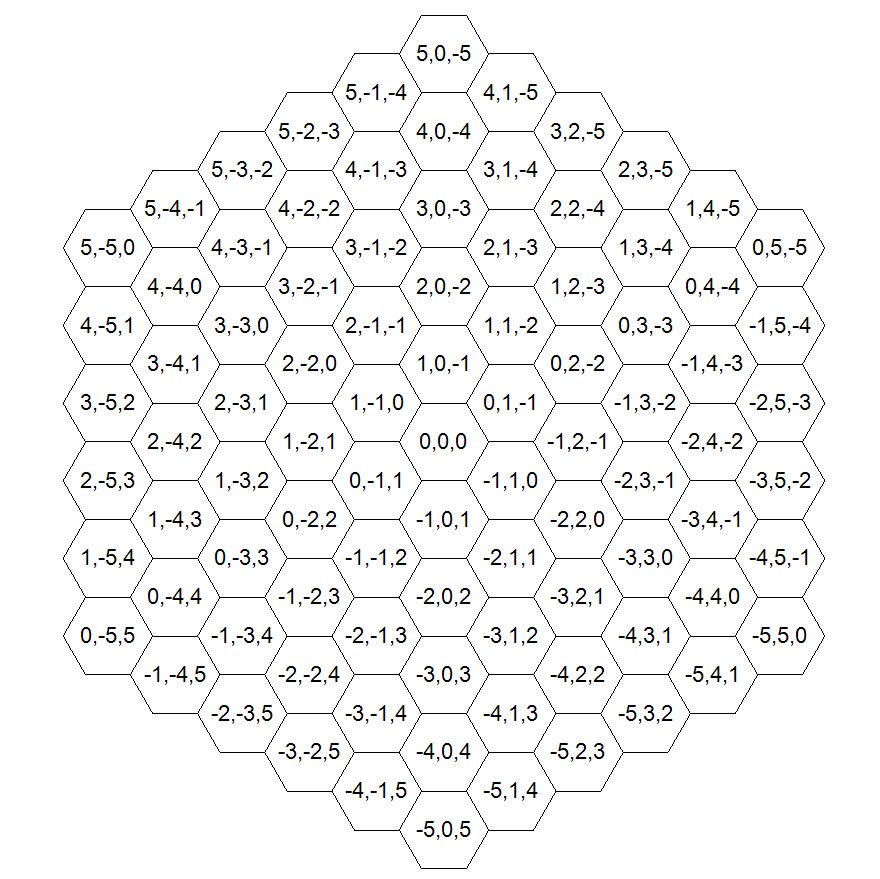
\includegraphics[width=1.1\linewidth]{HexCoord.png}
       \caption{Hexagonale Indizierung}
    \end{minipage}
    \hspace{.1\linewidth}% Abstand zwischen Bilder
    \begin{minipage}[t]{.4\linewidth} % [b] => Ausrichtung an \caption
       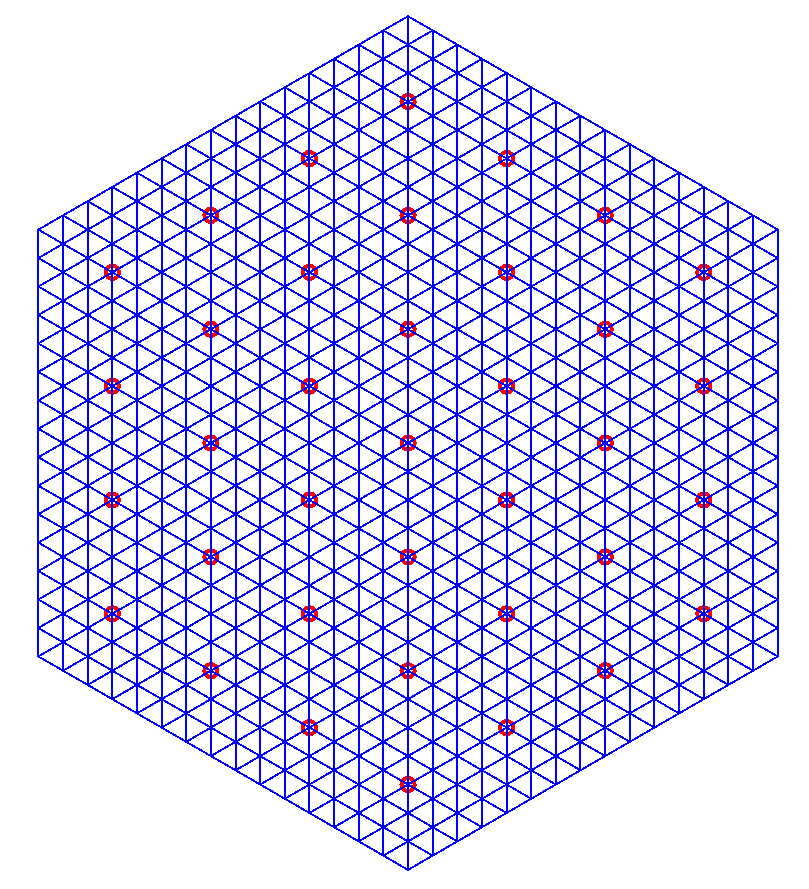
\includegraphics[width=\linewidth]{BoreHoleNet.png}
       \caption{Verteilung der Temperaturpunkte und der Erdsonden}
    \end{minipage}
 \end{figure}
 \textbf{Verhalten ohne Wärmezufuhr bzw. Wärmeentnahme:} Die Temperatur $T'$ im nächsten Zeitschritt wird durch die aktuelle Temperatur $T$ und die Temperaturdifferenzen zu den Nachbarpunkten $T_n$ bestimmt ($P$ und $P_n$ sind die Positionen der Punkte)
 \begin{align}
    T' = T + f\cdot \frac{\sum_{n=1}^{6} \frac{T-T_n}{|P,P_n|} }{6} 
 \end{align}
Der Faktor $f$ in obiger Formel sollte im wesentlichen von der Wärmeleitfähigkeit und Wärmekapazität abhängen und muss empirisch bestimmt werden. Der Abstand der Punkte ist bereits durch $\frac{1}{|P,P_n|}$ berücksichtigt.\\
Bei Punkten am Rand (weniger als 6 Nachbarn) wird die Umgebungstemperatur entsprechend berücksichtigt. Damit werden die Wärmeverluste des Erdsondenfelds nach außen simuliert, ebenso wie die Wärmeverluste nach oben und unten mit einer Temperaturabnahme der Temperaturpunkte selbst simuliert werden. $T'=T-f_v\cdot (T-T_{amb})$, wobei $f_v$ wieder empirisch bestimmt wird. Wenn der äußere Ring der Erdwärmesonden durch die Arbeit einer Wärmepumpe unter die Temperatur des umgebenden Erdreichs gesenkt wird, wird aus dem Wärmeverlust automatisch ein Wärmegewinn.\\
\textbf{Verhalten bei Wärmezufuhr bzw. Wärmeentnahme:} Die Temperaturänderung soll durch einen empirisch gewonnenen Faktor, der Sondenlänge und der Temperaturdifferenz zwischen der Erdsonde und dem die Sonde durchströmenden Wasser bestimmt werden. Für die nächste Sonde bei serieller Verbindung wird die durch die Energiezufuhr oder -entnahme veränderte Wassertemperatur verwendet.\\
Ein vorläufiger Test liefert zumindest anschaulich ansprechende Ergebnisse. Ob es gelingt, auf diese Art der gestellten Aufgabe gerecht zu werden, wird sich zeigen müssen.
\begin{figure}[h]
    \begin{minipage}[t]{.4\linewidth} % [b] => Ausrichtung an \caption
       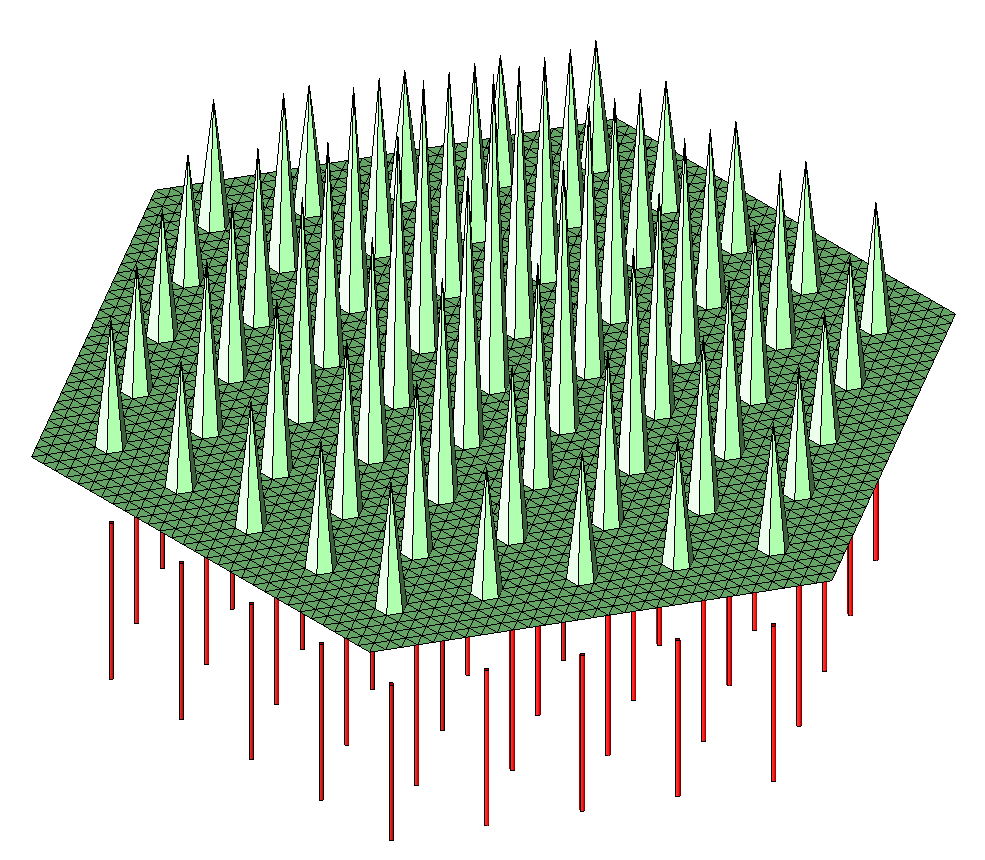
\includegraphics[width=\linewidth]{TempAt0.png}
       \caption{Temperaturverteilung unmittelbar nach Erwärmung durch die Edsonden}
       \label{TempAt0}
    \end{minipage}
    \hspace{.1\linewidth}% Abstand zwischen Bilder
    \begin{minipage}[t]{.4\linewidth} % [b] => Ausrichtung an \caption
       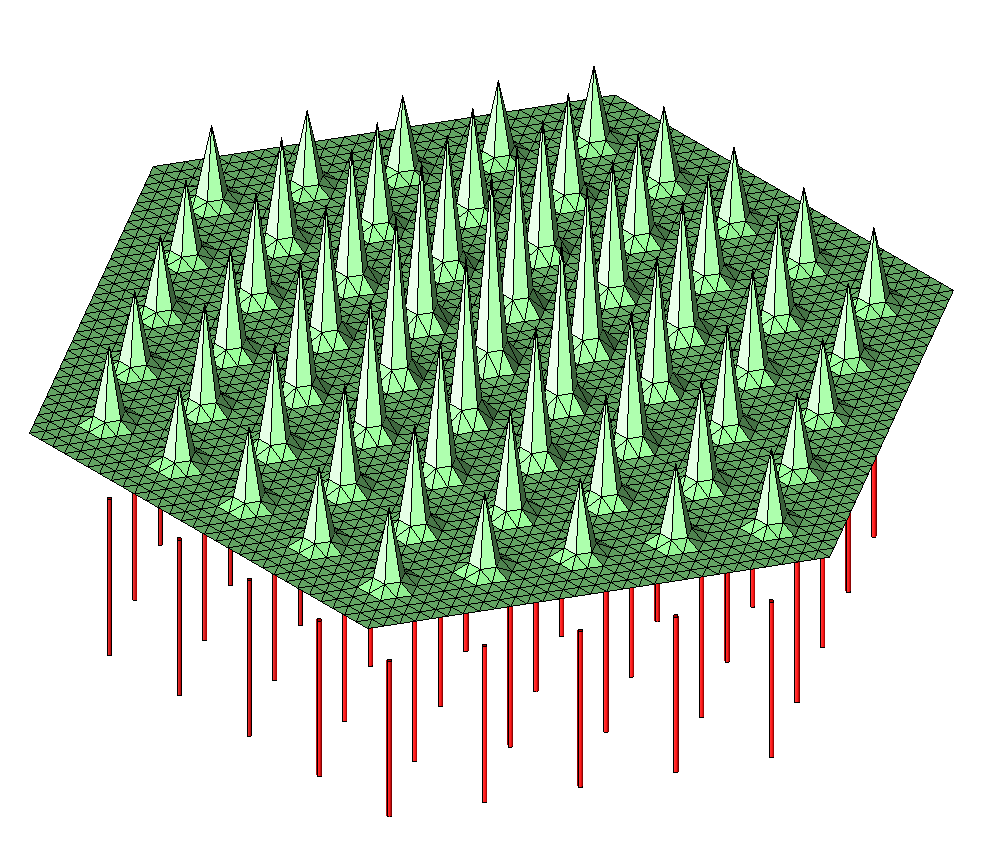
\includegraphics[width=\linewidth]{TempAt5.png}
       \caption{Temperaturverteilung kurze Zeit später}
       \label{TempAt5}
    \end{minipage}
 \end{figure}
 \begin{figure}[h]
    \begin{minipage}[t]{.4\linewidth} % [b] => Ausrichtung an \caption
       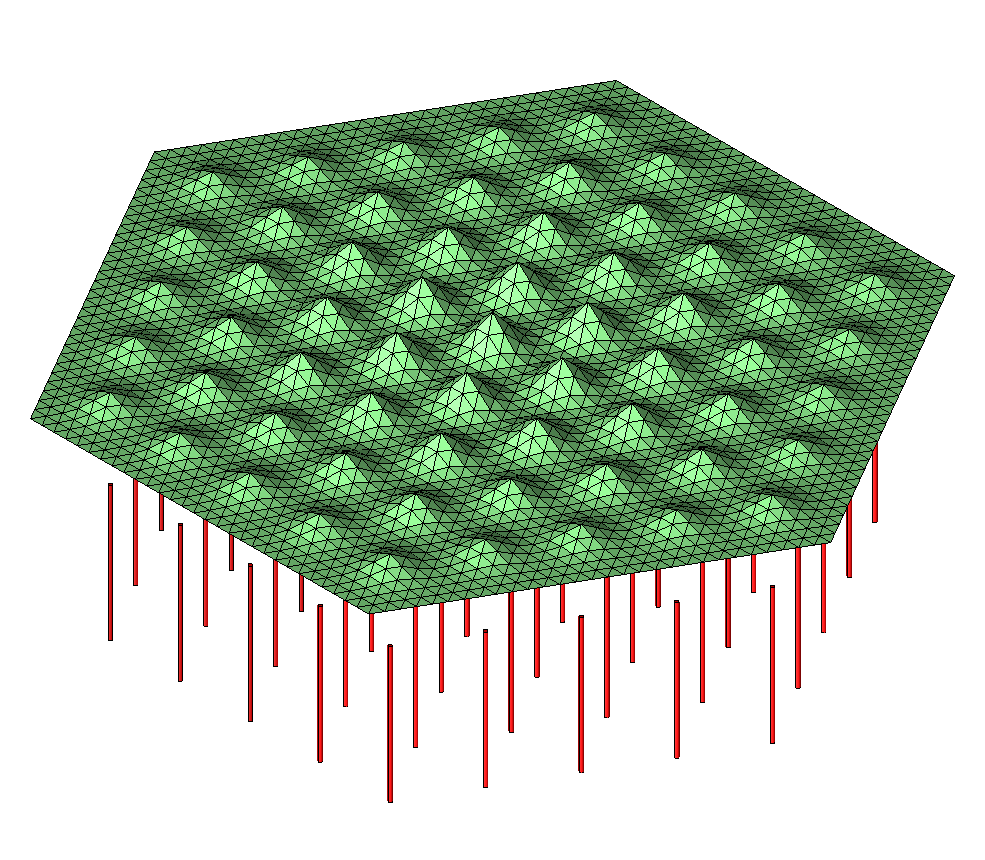
\includegraphics[width=\linewidth]{TempAt30.png}
       \caption{Temperaturverteilung nochmal später, die Erhöhung des Gesamtniveaus ist auf dem Bild kaum erkennbar}
       \label{TempAt30}
    \end{minipage}
    \hspace{.1\linewidth}% Abstand zwischen Bilder
    \begin{minipage}[t]{.4\linewidth} % [b] => Ausrichtung an \caption
       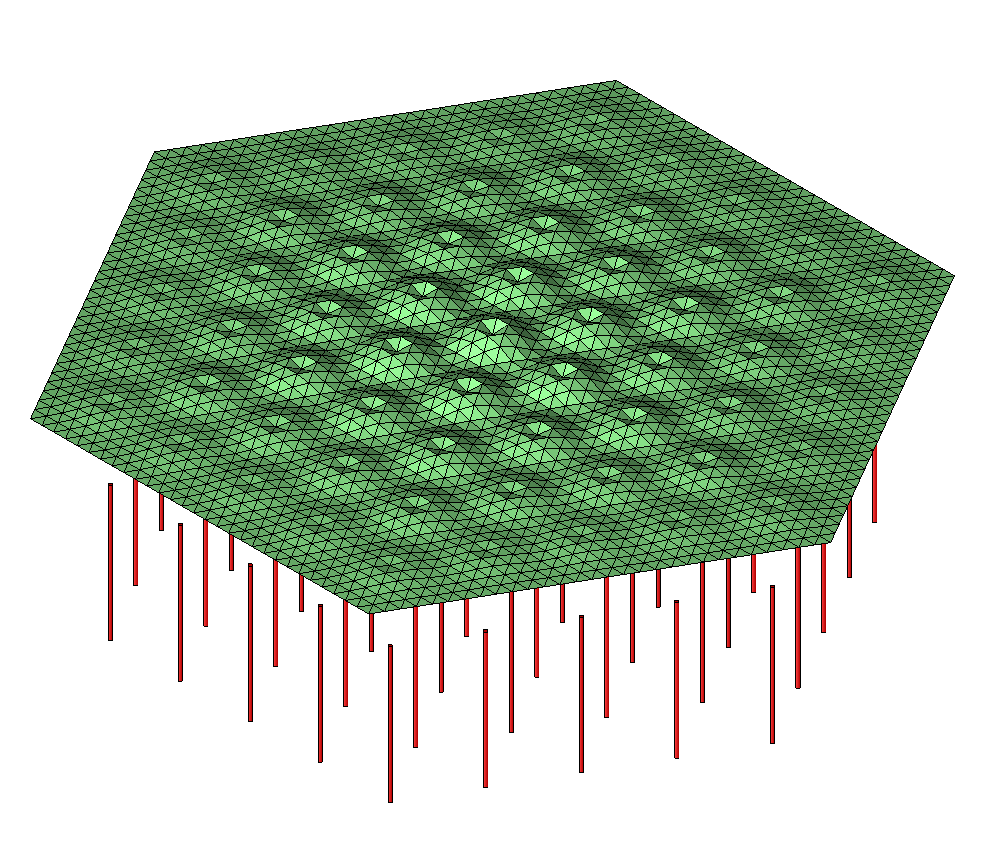
\includegraphics[width=\linewidth]{TempAt30m.png}
       \caption{Temperaturverteilung nachdem Wärme entnommen wurde}
       \label{TempAt30m}
    \end{minipage}
\end{figure}\\
Die Abbildungen \ref{TempAt0}, \ref{TempAt5}, \ref{TempAt30} und \ref{TempAt30m} zeigen das Temperaturprofil über den Erdsonden zu gewissen Zeitpunkten.
\end{document}